% !TEX program = xelatex
% 논문 USV_swarm_defense_EAAI_KR_real §4.3 "기하 휴리스틱 기준 방법" 식 (5)~(7) 해설 자료.
% 도판·수치는 make_figs_heur.py 가 figs/ 에 생성한다 (numbers_heur.json 참조).
% 예제는 군집화 해설(군집화_식1-4_해설.pdf)의 무리 1·2 를 그대로 이어받는다.
\documentclass[11pt,a4paper]{article}
\usepackage{kotex}
\usepackage{fontspec}
\setmainfont{TeX Gyre Termes}[Ligatures=TeX]
\setmainhangulfont{HCR Batang}[AutoFakeBold=2.0, AutoFakeSlant=0.2]
\setsanshangulfont{HCR Dotum}[AutoFakeBold=2.0, AutoFakeSlant=0.2]
\usepackage{amsmath, amssymb}
\usepackage{graphicx}
\usepackage{booktabs, array, multirow, tabularx}
\usepackage{xcolor}
\usepackage[margin=22mm]{geometry}
\usepackage{caption}
\usepackage{float}
\usepackage{tcolorbox}
\usepackage[hidelinks]{hyperref}
\graphicspath{{figs/}}
\setlength{\parskip}{4pt}
\setlength{\parindent}{0pt}
\linespread{1.15}
\captionsetup{font=small, labelfont=bf}
\renewcommand{\figurename}{그림}
\renewcommand{\tablename}{표}
\definecolor{navy}{HTML}{1F3A5F}
\definecolor{keybg}{HTML}{EEF3FA}
\definecolor{whybg}{HTML}{FFF6E5}
\newtcolorbox{keybox}[1][핵심]{colback=keybg, colframe=navy, title=#1, fonttitle=\bfseries, boxrule=0.6pt, left=6pt, right=6pt, top=4pt, bottom=4pt}
\newtcolorbox{whybox}[1][왜 이렇게 쓰나]{colback=whybg, colframe=orange!70!black, title=#1, fonttitle=\bfseries, boxrule=0.6pt, left=6pt, right=6pt, top=4pt, bottom=4pt}
\newcommand{\bfe}{\mathbf{e}}
\newcommand{\bfm}{\mathbf{m}}
\newcommand{\bfc}{\mathbf{c}}
\newcommand{\bfa}{\mathbf{a}}
\newcommand{\bfI}{\mathbf{I}}
\newcommand{\bft}{\mathbf{t}}
\newcommand{\rhat}{\hat{\mathbf{r}}}
\newcommand{\lamI}{\lambda_{\mathrm{I}}}
\newcommand{\lamL}{\lambda_{\mathrm{L}}}
\newcommand{\Lnet}{L_{\mathrm{net}}}

\title{\bfseries 기하 휴리스틱 기준 방법 --- 식 (5)--(7) 해설\\[4pt]
\large\mdseries USV 군집 방어 원고 (\texttt{USV\_swarm\_defense\_EAAI\_KR\_real}) \S4.3 보조 자료}
\author{}
\date{2026-09-20}

\begin{document}
\maketitle
\vspace{-14pt}

\begin{keybox}[이 자료의 목적과 위치]
\S4.3의 휴리스틱은 \S4.2가 만든 무리 요약($n_j$, $\bfc_j$)을 입력으로 받아, \textbf{기하 규칙만으로} "누가 어느 무리를 맡고, 그물벽을 어디에 놓는가"를 정하는 기준 방법이다.
세 식은 각각 (5)~\textbf{위협도와 요격점}, (6)~\textbf{배정 비용}, (7)~\textbf{그물벽 양 끝 경유점}이다.
예제는 군집화 해설(\texttt{군집화\_식1-4\_해설.pdf})의 결과 --- 무리 1 $\{n=2,\ \bfc_1=(-2155,-4601)\}$, 무리 2 $\{n=3,\ \bfc_2=(1432,3902)\}$ --- 를 그대로 이어받고, 방어정 $P=3$척을 추가한다.
모든 수치는 \texttt{make\_figs\_heur.py}로 계산했고 구현(\texttt{defense\_env.py}의 \texttt{\_compute\_assignment}, \texttt{heuristic\_pix})과 대조했다(부록~A).
\end{keybox}

\begin{figure}[H]
\centering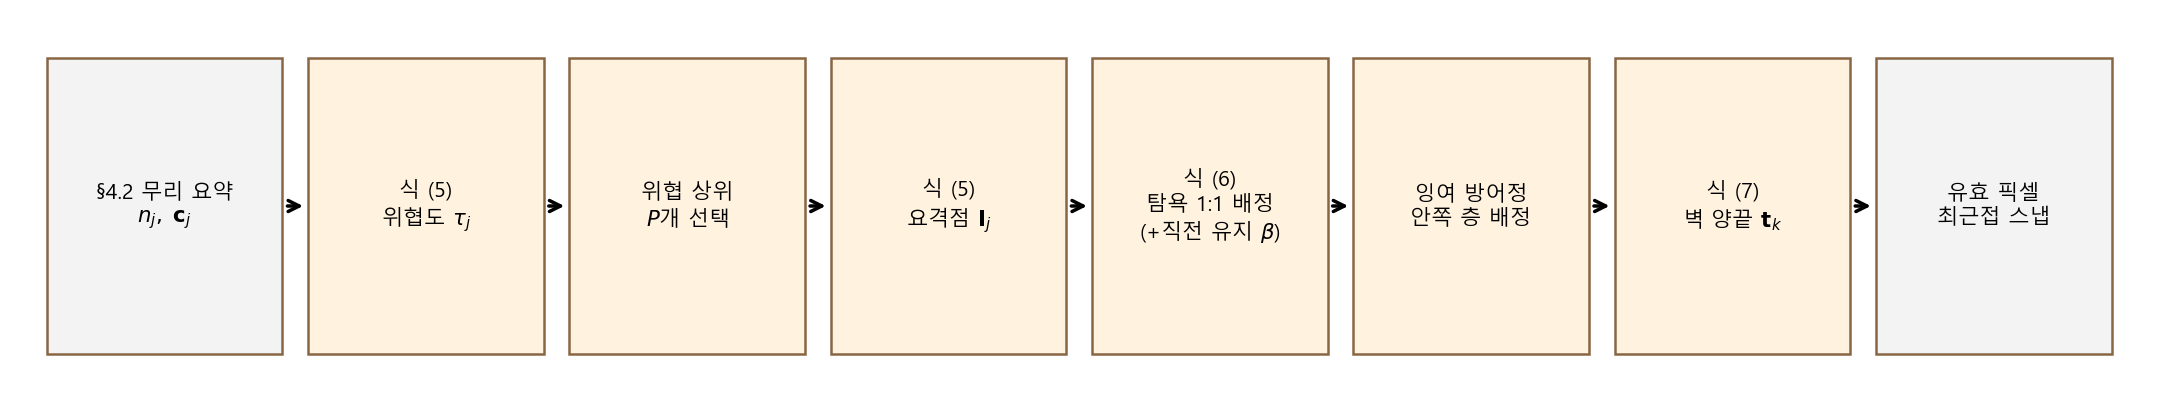
\includegraphics[width=\textwidth]{fig_h_pipeline.png}
\caption{\S4.3 파이프라인. 회색은 입·출력, 주황이 이 자료가 다루는 단계.}
\end{figure}

\section{휴리스틱의 역할 --- 왜 따로 두는가}

원고에서 휴리스틱은 세 가지 역할을 동시에 맡는다.
\begin{enumerate}
\item \textbf{비교 기준}(\S5 결과): 학습 정책이 "기하 상식"보다 나은지 재는 잣대.
\item \textbf{행동 복제(BC) 목표}(\S4.5): 학습 초기에 정책이 흉내 낼 교사. 그래서 휴리스틱의 출력은 정책과 \emph{같은 행동공간}(격자 픽셀)이어야 하고, 식~(7) 뒤의 "픽셀 스냅"이 그 다리다.
\item \textbf{배정 베이스}: 학습 정책도 "누가 어느 무리"는 이 휴리스틱 배정을 그대로 쓰고, 정책은 그 위에서 \emph{벽을 어디에 놓을지}만 학습한다(\texttt{learn\_assign=False}).
\end{enumerate}
따라서 \S4.3은 단순한 baseline 서술이 아니라, 학습 정책의 입력(배정 요격점 $\bfI_p$, 유효 마스크 $\mathcal V_p$)을 만드는 절이기도 하다.

\medskip
\textbf{예제 설정.} 모선 $\bfm=(0,0)$, 방어정 3척은 모선 함미 550 m 아래 한 줄: $\bfa_1=(-500,-550)$, $\bfa_2=(0,-550)$, $\bfa_3=(500,-550)$. 해역 반폭 $R_w=6300$ m, 적선 속력 $v_e=9$ m/s, 방어정 $v_a=6$ m/s(속력비 1.5).

\section{식 (5) --- 위협도와 요격점}

\begin{equation*}
\tau_j = n_j\cdot\mathrm{clip}\!\Big(1-\frac{\lVert\bfc_j-\bfm\rVert}{R_w},\ 0.05,\ 1\Big), \qquad
\bfI_j = \bfc_j + \lamI\,(\bfm-\bfc_j),\quad \lamI=0.55 \tag{5}
\end{equation*}

\subsection{위협도 $\tau_j$ --- "몇 척이, 얼마나 가까이"}

\textbf{구조.} 척수 $n_j$ $\times$ 근접도. 근접도는 무리 중심--모선 거리를 해역 반폭으로 나눠 1에서 뺀 값이라, 모선 위에서 1, 해역 가장자리($R_w$)에서 0이 되는 선형 감쇠다(그림~\ref{fig:threat}).

\textbf{하한 0.05.} 해역 가장자리 밖($d>R_w$)의 무리도 근접도가 0이 되면 $\tau_j=0$이 되어 척수 정보가 사라진다. 하한을 두면 먼 무리도 "척수 $\times$ 0.05"만큼의 위협을 가져 위협 순위에서 척수 순으로 줄을 선다.

\begin{figure}[H]
\centering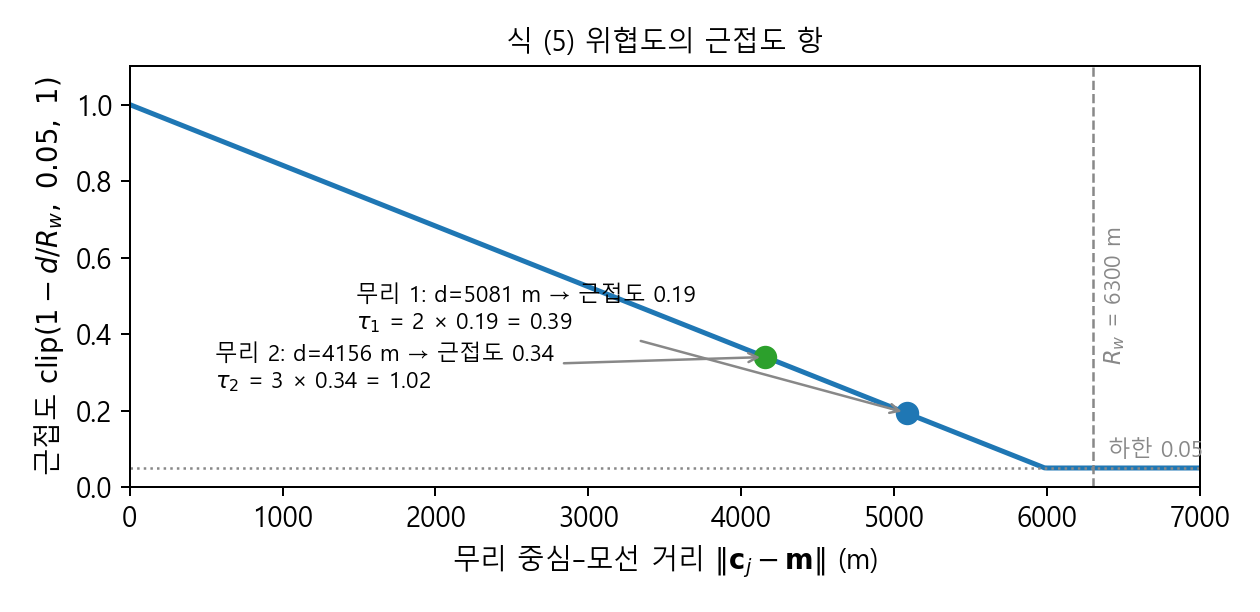
\includegraphics[width=0.75\textwidth]{fig_h_threat.png}
\caption{근접도 항. 예제 두 무리의 위치와 위협도.}\label{fig:threat}
\end{figure}

\textbf{예제.}
무리 1: $d=5081$ m $\to$ 근접도 $1-5081/6300=0.194$, $\tau_1 = 2\times0.194 = 0.39$.
무리 2: $d=4156$ m $\to$ 근접도 $0.340$, $\tau_2 = 3\times0.340 = 1.02$.
무리 2가 더 많고 더 가까우므로 위협 1순위.

\begin{whybox}[왜 접근 속도나 각도 퍼짐은 안 쓰나]
휴리스틱은 "기하 규칙만으로"가 설계 조건이다. 척수와 거리는 기하이고, 접근 속도 $v^{\rm app}_j$와 퍼짐 $\Delta\vartheta_j$는 학습 정책의 관측으로만 넘긴다. 이렇게 두면 \S5의 비교가 "정보량 차이"가 아니라 "결정 규칙 차이"가 된다(원고 \S4.3 마지막 문단).
\end{whybox}

\subsection{요격점 $\bfI_j$ --- 무리 중심과 모선 사이 어디에 벽을 세우나}

\textbf{구조.} 무리 중심 $\bfc_j$에서 모선 $\bfm$을 향해 선분의 $\lamI$ 비율만큼 옮긴 점. $\lamI=0$이면 무리 중심, $1$이면 모선.

\begin{figure}[H]
\centering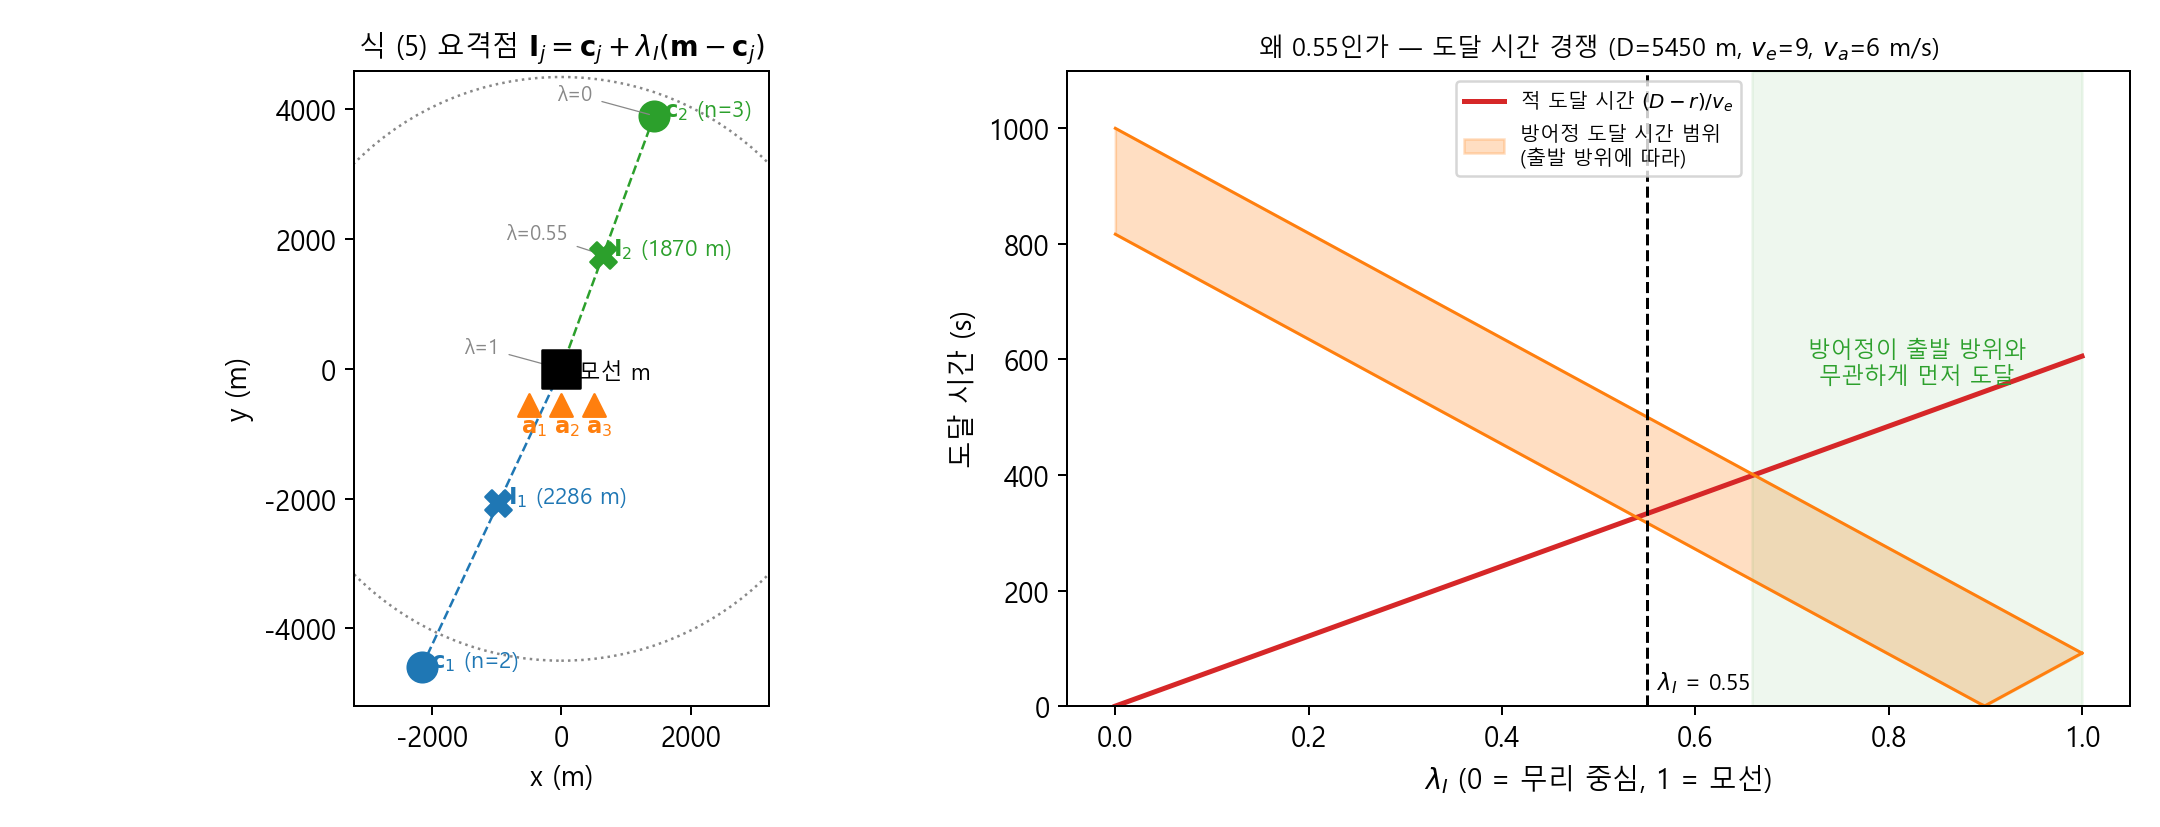
\includegraphics[width=\textwidth]{fig_h_intercept.png}
\caption{(a) 예제의 요격점. (b) 도달 시간 경쟁: 적은 5450 m에서 출발해 반경 $r=(1-\lamI)D$ 까지 $(D-r)/v_e$, 방어정은 모선 550 m 옆에서 출발해 $|r\mp550|/v_a$. 빨간 선이 주황 띠 아래에 있으면 적이 먼저 온다.}\label{fig:intercept}
\end{figure}

\begin{whybox}[왜 0.55인가 --- 방어정이 적보다 느리다]
방어정($v_a=6$)이 적($v_e=9$)보다 느리므로 요격점은 "방어정이 적보다 먼저 닿는 곳"이어야 의미가 있다. 적 출발 거리 $D=5450$ m, 방어정 출발 위치를 모선 550 m 옆으로 놓고 도달 시간을 비교하면(그림~\ref{fig:intercept}b):
\begin{itemize}
\item 방어정이 요격점 쪽 방위에서 출발(최선)하면 $\lamI\ge0.54$, 즉 모선 반경 약 2.5 km 안쪽부터 먼저 닿는다.
\item 반대쪽에서 출발(최악)하면 $\lamI\ge0.66$, 약 1.9 km 안쪽이라야 한다.
\end{itemize}
$\lamI=0.55$는 최선 경계에 맞춘 값으로, $D=5450$일 때 요격점 반경 $0.45\times5450\approx2450$ m다(구현 주석 "모선 반경 $\sim$2.4 km 안쪽"). 배정(\S3)이 "요격점에 가장 가까운 배"를 고르므로 실제로는 최선 쪽에 가깝고, 그물벽은 요격점을 지나 450 m 폭으로 깔리므로 약간의 여유가 있다.
더 안쪽(예: 0.7)으로 두면 항상 먼저 닿지만 모선 근접 반경 $r_{\min}=400$ m와 충돌 회피 반경에 가까워져 전개 공간이 좁아진다.
\end{whybox}

\textbf{예제.} $\bfI_2 = \bfc_2 + 0.55(\bfm-\bfc_2) = (1432,3902)\times0.45 = (644,\ 1756)$, 모선에서 1870 m. $\bfI_1 = (-970,\ -2070)$, 2286 m.

\section{식 (6) --- 배정: 누가 어느 무리를 맡나}

\begin{equation*}
\tilde d_{pj} = d_{pj} - \beta\cdot\mathbb 1[\,j = j_p^{\rm prev}\,], \qquad d_{pj} = \lVert\bfa_p-\bfI_j\rVert \tag{6}
\end{equation*}

\textbf{절차.} (i) 위협도 상위 $P$개 활성 무리를 대상으로 잡는다. (ii) 방어정 $p$와 무리 $j$의 비용 $\tilde d_{pj}$ 행렬을 만든다. (iii) \textbf{탐욕 1:1}: 행렬에서 가장 작은 칸을 고르고 그 행(배)과 열(무리)을 지우기를 반복. (iv) 남는 배는 잉여 배정(\S\ref{sec:surplus}).

\subsection{기본 비용 $d_{pj}$ --- 요격점까지의 거리}

\textbf{예제.} 위협 순 대상 = \{무리 2, 무리 1\}. 거리 행렬(m):
\begin{table}[H]
\centering\small
\begin{tabular}{c c c}
\toprule
 & 무리 2 ($\bfI_2$) & 무리 1 ($\bfI_1$) \\
\midrule
$\bfa_1$ & 2574 & \textbf{1591} \\
$\bfa_2$ & 2394 & 1803 \\
$\bfa_3$ & \textbf{2310} & 2115 \\
\bottomrule
\end{tabular}
\end{table}
탐욕 1단계: 최소 1591 $\to$ $\bfa_1\to$ 무리 1. $\bfa_1$ 행과 무리 1 열 제거. 2단계: 남은 최소 2310 $\to$ $\bfa_3\to$ 무리 2. $\bfa_2$는 잉여(그림~\ref{fig:assign}a).

\begin{whybox}[왜 헝가리안(최적 매칭)이 아니라 탐욕인가]
$P=3$, $\hat C\le4$의 $3\times4$ 행렬이라 최적 매칭과 탐욕의 차이가 실질적으로 없고, 탐욕은 $N$개 월드를 벡터화해 한 번에 돌리기 쉽다(구현: \texttt{argmin} 반복 $\min(P,K)$회). 더 중요한 이유는 다음의 $\beta$가 비용을 크게 왜곡하므로 어차피 "최적 거리 매칭"이 목표가 아니라는 점이다.
\end{whybox}

\subsection{유지 보너스 $\beta$ --- 배정이 매 결정마다 뒤집히지 않게}

\textbf{문제.} 배와 적이 움직이면 거리 순위가 조금씩 바뀐다. 거리만 보면 결정마다 배정이 뒤바뀌고(churn), 반쯤 깐 그물벽을 버리고 다른 무리로 이동해 벽도 이동도 낭비된다. 원고: "전개 중 담당이 바뀌면 이동과 그물이 회수되지 않기 때문."

\textbf{해법.} 직전 결정에서 $p$가 맡았던 무리 $j_p^{\rm prev}$와의 쌍에만 비용을 $\beta=6000$ m 깎는다. 지시함수 $\mathbb 1[\cdot]$은 그 조건이 참이면 1, 아니면 0.

\textbf{예제.} 직전 결정이 $\bfa_2\to$무리 1, $\bfa_1\to$무리 2였다고 하자(그 뒤 배·적이 움직여 지금은 거리만 보면 $\bfa_1\to$무리 1이 더 가깝다).
\begin{table}[H]
\centering\small
\begin{tabular}{c c c}
\toprule
 & 무리 2 & 무리 1 \\
\midrule
$\bfa_1$ & $2574-6000=\mathbf{-3426}$ & 1591 \\
$\bfa_2$ & 2394 & $1803-6000=\mathbf{-4197}$ \\
$\bfa_3$ & 2310 & 2115 \\
\bottomrule
\end{tabular}
\end{table}
탐욕: $-4197\to\bfa_2\to$무리 1, $-3426\to\bfa_1\to$무리 2. 직전 배정이 그대로 유지되고 $\bfa_3$이 잉여가 된다(그림~\ref{fig:assign}b).

\begin{whybox}[왜 6000 m인가 --- 거의 무조건 유지]
해역 반폭이 6300 m이므로 $\beta=6000$은 "직전 무리가 아직 대상이면 거리와 무관하게 유지"에 가깝다. 구현 주석의 실측: churn 26$\to$9\%, 포획 1906$\to$1984. 유지가 풀리는 경우는 직전 무리가 위협 상위 $P$개에서 빠졌을 때(전멸·병합)뿐이다.
원고 식~(6)에는 생략되어 있지만, 구현은 "직전 무리가 여전히 대상 집합에 있을 때만" 보너스를 준다(\texttt{prev\_is\_target}).
\end{whybox}

\subsection{잉여 방어정 --- 안쪽 층}\label{sec:surplus}

활성 무리가 $P$보다 적으면 1:1 뒤 배가 남는다. 남는 배를 놀리지 않고 \textbf{부하} $n_j/(1+\text{배정된 배 수})$가 가장 큰 무리에 덧붙이되, 같은 요격점에 겹치면 벽이 중복되므로
\begin{itemize}
\item 요격점 비율을 $\lamI + \lamL\cdot(\text{기존 배정 수})$, $\lamL=0.18$로 \textbf{모선 쪽 한 층 안쪽}에 두고(종심 방어),
\item 모선 기준 방위를 $\pm40^\circ$ 교대로 틀어 두 배가 같은 방위선 위를 앞뒤로 달리지 않게 한다(구현 주석: 틀지 않으면 집중 포메이션에서 아군 충돌 0$\to$9).
\end{itemize}

\textbf{예제.} 부하: 무리 1 $=2/(1+1)=1.0$, 무리 2 $=3/(1+1)=1.5$ $\to$ 무리 2. $\lambda=0.55+0.18=0.73$, 방위 $-40^\circ$ $\to$ 층 요격점 $(973,\ 559)$, 모선에서 1121 m.

\begin{figure}[H]
\centering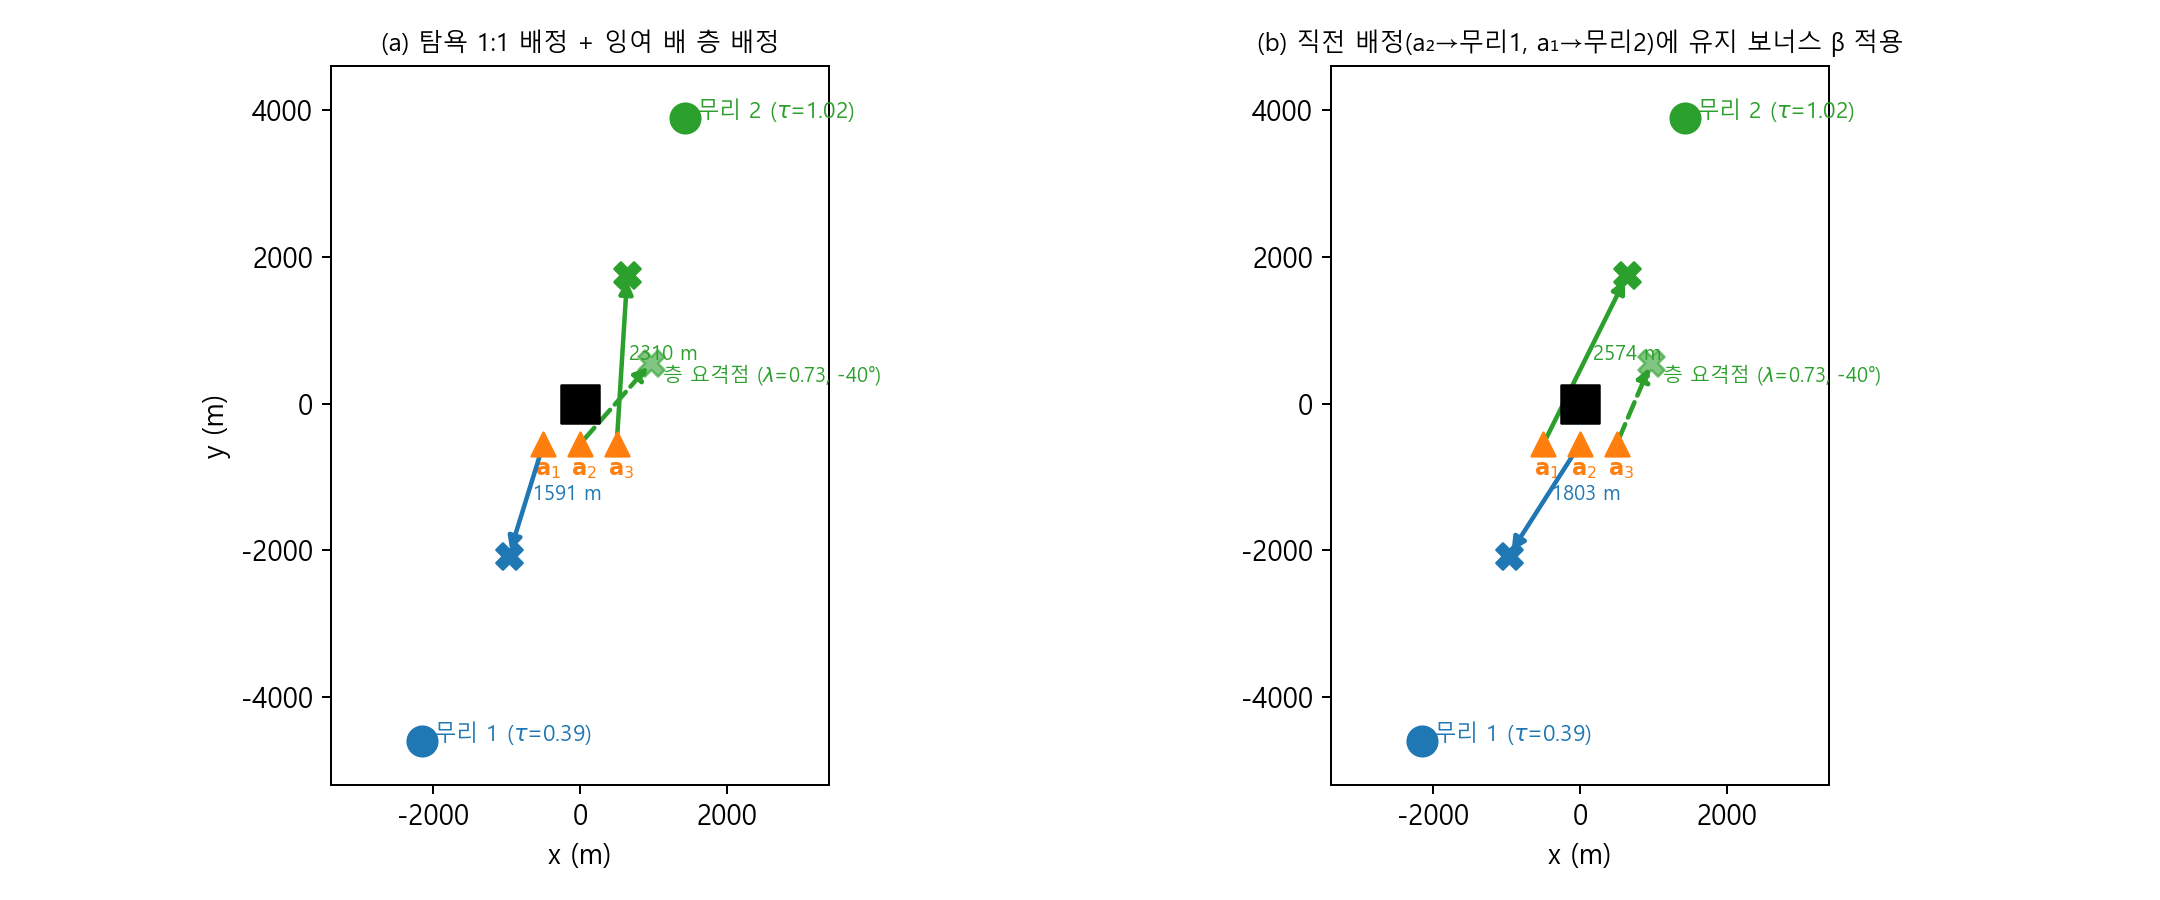
\includegraphics[width=\textwidth]{fig_h_assign.png}
\caption{배정 결과. 실선 = 1:1 배정, 점선 = 잉여 배의 층 배정. (a)와 (b)는 직전 배정만 다르다.}\label{fig:assign}
\end{figure}

\section{식 (7) --- 경유점: 그물벽의 양 끝}

\begin{equation*}
\bft_k = \bfI + \Big(k - \tfrac{K-1}{2}\Big)\Lnet\,\rhat^{\perp}, \qquad k=0,\dots,K-1,\quad K=2,\ \Lnet=450\text{ m} \tag{7}
\end{equation*}

\textbf{구조.} 그물벽은 요격점 $\bfI$를 가운데 둔 길이 $\Lnet$의 선분이고, 방향은 접근 방향에 \textbf{수직}이다. $\rhat$은 모선$\to$요격점 단위벡터(= 적이 오는 방향의 반대), $\rhat^\perp$은 그에 수직인 단위벡터. $K=2$이면 $k-\frac{K-1}{2} = \pm\frac12$이므로 $\bft_{0,1} = \bfI \mp \frac{\Lnet}{2}\rhat^\perp$, 즉 요격점 양옆 225 m.

\textbf{예제}(무리 2). $\rhat = \bfI_2/\lVert\bfI_2\rVert = (0.345, 0.939)$, $\rhat^\perp = (-0.939, 0.345)$.
$\bft_0 = (644,1756) - 225\,\rhat^\perp = (856,\ 1678)$, $\bft_1 = (433,\ 1833)$. 두 점 거리 450 m.

\begin{whybox}[왜 수직인가]
적은 무리 중심에서 모선으로, 즉 $-\rhat$ 방향으로 온다. 벽이 이 방향에 수직이면 벽의 투영 폭이 최대(450 m)가 되어 가장 많은 적선 궤적을 가로지른다. 평행이면 투영 폭이 0이다. 무리의 각도 퍼짐이 크면 더 긴 벽이 필요하지만, 휴리스틱은 $\Lnet$ 고정이다 --- 학습 정책은 두 끝점을 자유롭게 찍어 이를 넘을 수 있다.
\end{whybox}

\subsection{픽셀 스냅과 유효 마스크 --- 정책과 같은 행동공간}

학습 정책은 좌표가 아니라 $50\times50$ 격자(픽셀 한 변 $\ell=252$ m)의 픽셀을 고른다. 휴리스틱도 같은 공간에서 비교·BC 하려면 $\bft_k$를 픽셀로 바꿔야 한다.
\begin{enumerate}
\item 방어정 $p$의 \textbf{유효 픽셀} $\mathcal V_p$(\S4.4.3): 환형 요격 구역 $400\le r\le4500$ m $\cap$ 육지 밖 $\cap$ 요격점 반경 3000 m 안 $\cap$ 요격점 방위 $\pm60^\circ$ 안.
\item $\bft_0$을 $\mathcal V_p$ 안에서 \textbf{최근접 픽셀 중심}으로 스냅하고, \textbf{간격 제약} --- 첫 픽셀에서 $r_{\rm dup}=200$ m 이상 $1.5\Lnet=675$ m 이하 --- 을 만족하는 픽셀 중에서 $\bft_1$을 스냅한다.
\end{enumerate}

\begin{figure}[H]
\centering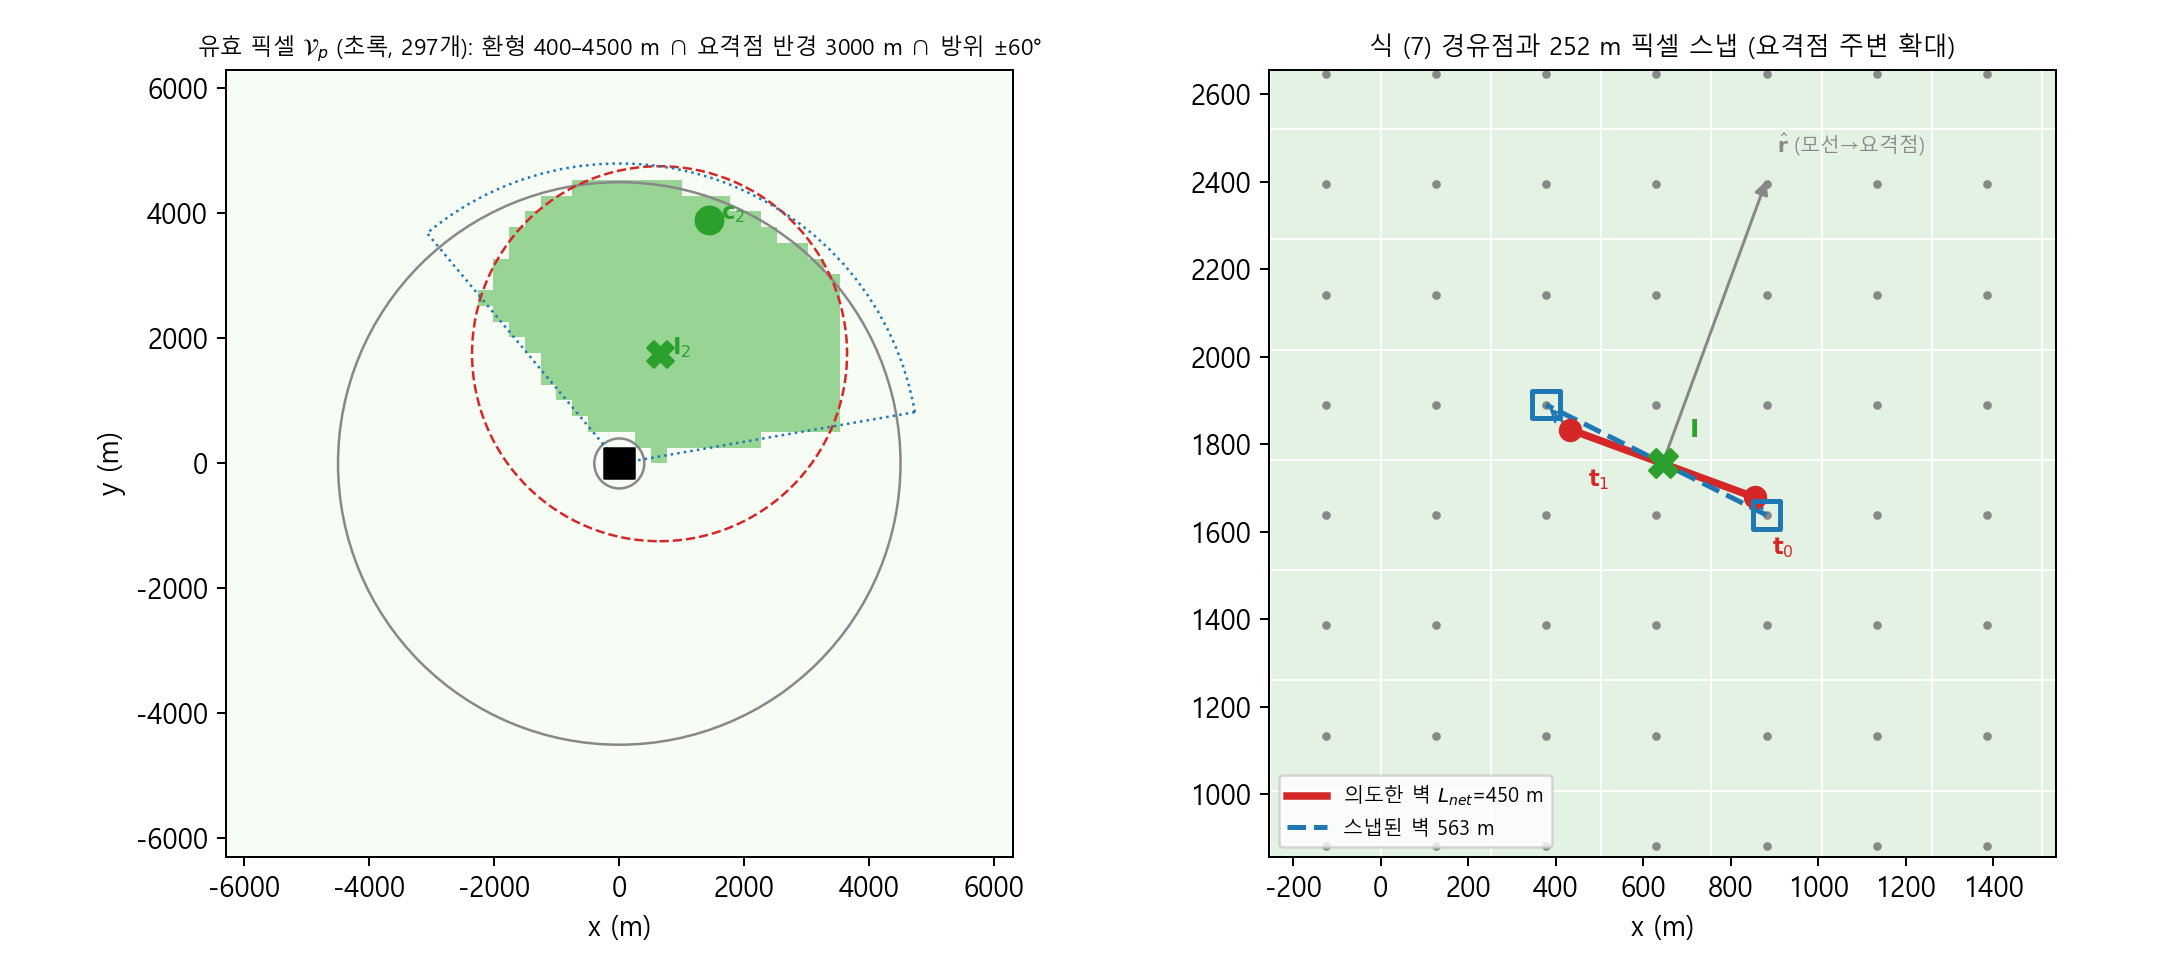
\includegraphics[width=\textwidth]{fig_h_waypoint.png}
\caption{(a) 예제 방어정의 유효 픽셀(297개). (b) 요격점 주변 확대: 의도한 벽(빨강)과 스냅된 벽(파랑).}\label{fig:wp}
\end{figure}

\textbf{예제.} 스냅 결과 $(882,1638)$, $(378,1890)$ --- 두 픽셀 중심 거리 \textbf{563 m}로 의도한 450 m보다 길다. 픽셀이 252 m 단위라 양 끝이 각각 최대 $126\sqrt2\approx178$ m 튈 수 있기 때문이다. 563 m는 간격 제약 $[200, 675]$ m 안이므로 허용된다.

\begin{whybox}[스냅이 만드는 문제와 간격 제약의 역할]
구현 주석의 실측: 스냅 뒤 벽 길이 중앙값 504 m, 450 m 초과율 66.7\%. 그물은 물리적으로 450 m까지만 깔리므로 두 점이 그보다 멀면 벽이 둘째 점에 닿지 못한 채 끝난다. 간격 상한 $1.5\Lnet$은 이 초과를 한계 안에 묶고, 하한 $r_{\rm dup}$는 두 점이 같은 자리에 겹쳐 길이 0의 벽이 되는 것을 막는다. 정책과 휴리스틱이 \emph{같은} 유효 마스크와 간격 제약을 쓰므로, 원고 문장대로 "두 방법의 행동공간은 같다" --- 이것이 BC 목표로 쓸 수 있는 전제이기도 하다(휴리스틱 픽셀이 정책의 마스크 밖이면 로그확률이 $-\infty$가 되어 BC 손실이 정의되지 않는다).
\end{whybox}

\section{휴리스틱이 못 보는 것 --- 학습 정책과의 차이}

원고 \S4.3 마지막 문단의 요지를 예제로 풀면:
\begin{table}[H]
\centering\small
\begin{tabularx}{\textwidth}{>{\raggedright\arraybackslash}p{0.26\textwidth} >{\raggedright\arraybackslash}X}
\toprule
휴리스틱이 고려하지 않는 것 & 예제에서의 의미 \\
\midrule
다른 방어정의 벽 & $\bfa_3$과 $\bfa_2$가 모두 무리 2를 맡지만, 층 배정($\lamL$, $\pm40^\circ$)이라는 고정 규칙으로만 떨어뜨린다. 서로의 벽 위치를 보고 빈틈을 메우지는 않는다. \\
파상 공격의 뒤 단 & 무리 2 뒤에 두 번째 단이 있어도 요격점은 첫 단 중심만 본다. \\
지형의 길목 & 유효 마스크가 육지를 빼 주긴 하지만, 적이 지나갈 수밖에 없는 해협을 골라 벽을 놓지는 않는다. \\
무리의 퍼짐·접근 속도 & $\Delta\vartheta_j$, $v^{\rm app}_j$는 관측으로만 넘어가고 휴리스틱은 쓰지 않는다. \\
\bottomrule
\end{tabularx}
\end{table}
학습 정책은 같은 배정·같은 유효 마스크 위에서 점수맵으로 해면 전체 후보를 한꺼번에 비교하므로, \S5의 차이는 "무엇을 볼 수 있느냐"가 아니라 "어떻게 고르느냐"의 차이다.

\section{자주 헷갈리는 점 정리}

\begin{table}[H]
\centering\small
\begin{tabularx}{\textwidth}{>{\raggedright\arraybackslash}p{0.34\textwidth} >{\raggedright\arraybackslash}X}
\toprule
질문 & 답 \\
\midrule
$\tau_j$ 하한 0.05는 왜 0이 아닌가? & 0이면 먼 무리들이 전부 동률 0이 되어 척수 순위가 사라진다. 0.05는 "척수 $\times$ 0.05"로 순위를 남긴다. \\
$\lamI$는 무리 쪽 비율인가 모선 쪽 비율인가? & 모선 쪽. $\bfI = \bfc + \lamI(\bfm-\bfc)$이므로 $\lamI$가 클수록 모선에 가깝다. \\
$\beta$를 빼는데 비용이 음수가 돼도 되나? & 된다. 탐욕은 대소만 비교하므로 절대값은 무관하다. 음수 = "거의 무조건 먼저 선택". \\
$j_p^{\rm prev}$가 사라진 무리면? & 대상 집합에 없으므로 보너스가 적용되지 않고 거리로만 배정된다. \\
$K=2$인데 왜 일반식으로 쓰나? & $K$개 경유점을 벽을 따라 등간격으로 놓는 일반형. 학습 정책도 결정마다 그물벽 하나(끝점 2개)를 놓으므로 $K=2$로 맞춘 것. \\
$\rhat^\perp$의 방향(좌/우)은? & 어느 쪽이든 $\bft_0$, $\bft_1$이 서로 바뀔 뿐 벽은 같다. 구현은 $(-r_y, r_x)$. \\
스냅된 벽이 450 m보다 길면? & 그물은 450 m까지만 깔린다. 간격 제약 상한 $1.5\Lnet=675$ m가 초과를 한계 안에 묶고, 그 안의 초과분은 벽 끝이 짧아지는 것으로 흡수된다. \\
\bottomrule
\end{tabularx}
\end{table}

\appendix
\section{원고 식 $\leftrightarrow$ 구현 코드 대응}

배정은 \texttt{boatattack\_sim/env/defense\_env.py}의 \texttt{\_compute\_assignment}, 경유점·스냅은 같은 파일의 \texttt{heuristic\_pix}, 파라미터는 \texttt{env/config.py}.
\begin{table}[H]
\footnotesize
\begin{tabularx}{\textwidth}{>{\raggedright\arraybackslash}p{0.2\textwidth} >{\raggedright\arraybackslash}X >{\raggedright\arraybackslash}p{0.19\textwidth}}
\toprule
원고 & 코드 & 비고 \\
\midrule
식 (5) 근접도 & \texttt{close = np.clip(1.0 - md / self.world\_half, 0.05, 1.0)} & \texttt{world\_half} $=R_w$ \\
식 (5) $\tau_j$ & \texttt{threat = np.where(active, cnt * close, -1.0)} & 비활성 무리 $=-1$ \\
식 (5) $\bfI_j$ & \texttt{I = cent + t * (c - cent)}; \texttt{t = assign\_intercept\_t = 0.55} & \\
상위 $P$개 대상 & \texttt{topP = np.argsort(-threat)[:, :P]}; \texttt{target \&= active} & \\
식 (6) $d_{pj}$ & \texttt{cost = np.hypot(a\_pos - I)}; 비대상·사망 $=$ \texttt{BIG} & \\
식 (6) $\beta$ & \texttt{cost[...] -= assign\_sticky\_bonus (6000)}, 단 \texttt{prev\_is\_target} 일 때만 & 원고엔 조건 생략 \\
탐욕 1:1 & \texttt{for \_ in range(min(P, K)): argmin $\to$ 행·열 BIG} & \\
잉여 배 층 & \texttt{load = cnt/(1+nass)}; \texttt{tl = t + assign\_layer\_dt(0.18)·nass}; \texttt{assign\_layer\_dbear = 40} 교대 회전 & 원고 $\lamL$, $\pm40^\circ$ \\
식 (7) $\rhat^\perp$, $\bft_k$ & \texttt{perp = (-rad[1], rad[0])}; \texttt{off = (k-(K-1)/2)*net\_max\_len}; \texttt{pt = I + perp*off} & \texttt{net\_max\_len} $=450$ \\
유효 마스크·스냅 & \texttt{avail = \_cnn\_valid\_mask()}; \texttt{d2 = where(avail, ...)}; \texttt{argmin}; \texttt{disk\_exclude(cnn\_dup\_r=200)}; \texttt{reach\_keep(net\_max\_len·cnn\_reach\_slack)} & \S4.4.3 $\mathcal V_p$, 간격 $[r_{\rm dup}, 1.5\Lnet]$ \\
\bottomrule
\end{tabularx}
\end{table}

\end{document}
